\documentclass[dvipdfmx]{jarticle}
\usepackage{graphicx}
\usepackage[top=30truemm,bottom=30truemm,left=25truemm,right=25truemm]{geometry}
\usepackage{listings,jvlisting}
\usepackage{url}

\lstset{
  basicstyle={\ttfamily},
  identifierstyle={\small},
  commentstyle={\smallitshape},
  keywordstyle={\small\bfseries},
  ndkeywordstyle={\small},
  stringstyle={\small\ttfamily},
  frame={tb},
  breaklines=true,
  columns=[l]{fullflexible},
  numbers=left,
  xrightmargin=0zw,
  xleftmargin=3zw,
  numberstyle={\scriptsize},
  stepnumber=1,
  numbersep=1zw,
  lineskip=-0.5ex
}

\makeatletter
\newcommand{\subsubsubsection}{\@startsection{paragraph}{4}{\z@}%
  {1.0\Cvs \@plus.5\Cdp \@minus.2\Cdp}%
  {.1\Cvs \@plus.3\Cdp}%
  {\reset@font\sffamily\normalsize}
}
\makeatother
\setcounter{secnumdepth}{4}

\begin{document}
\begin{titlepage}
    \begin{center}
        {\huge 情報科学実験C 中間レポ―ト}
        \vspace{180pt}\\
        \begin{tabular}{rl}
            氏名 & 山久保孝亮\\
            所属 & 大阪大学基礎工学部情報科学科ソフトウェア科学コース\\
            メールアドレス & u327468b@ecs.osaka-u.ac.jp\\
            学籍番号 & 09B22084\\
            提出日 & \today\\
        \end{tabular}
    \end{center}
\end{titlepage}
\section{Tiny-ProcessorとC-Processorのデータパスの違い}
以下の図1,2はそれぞれTiny-ProcessorとC-Processorのデータパスである.
\begin{figure}[h]
  \centering
  \begin{minipage}[b]{0.49\columnwidth}
      \centering
      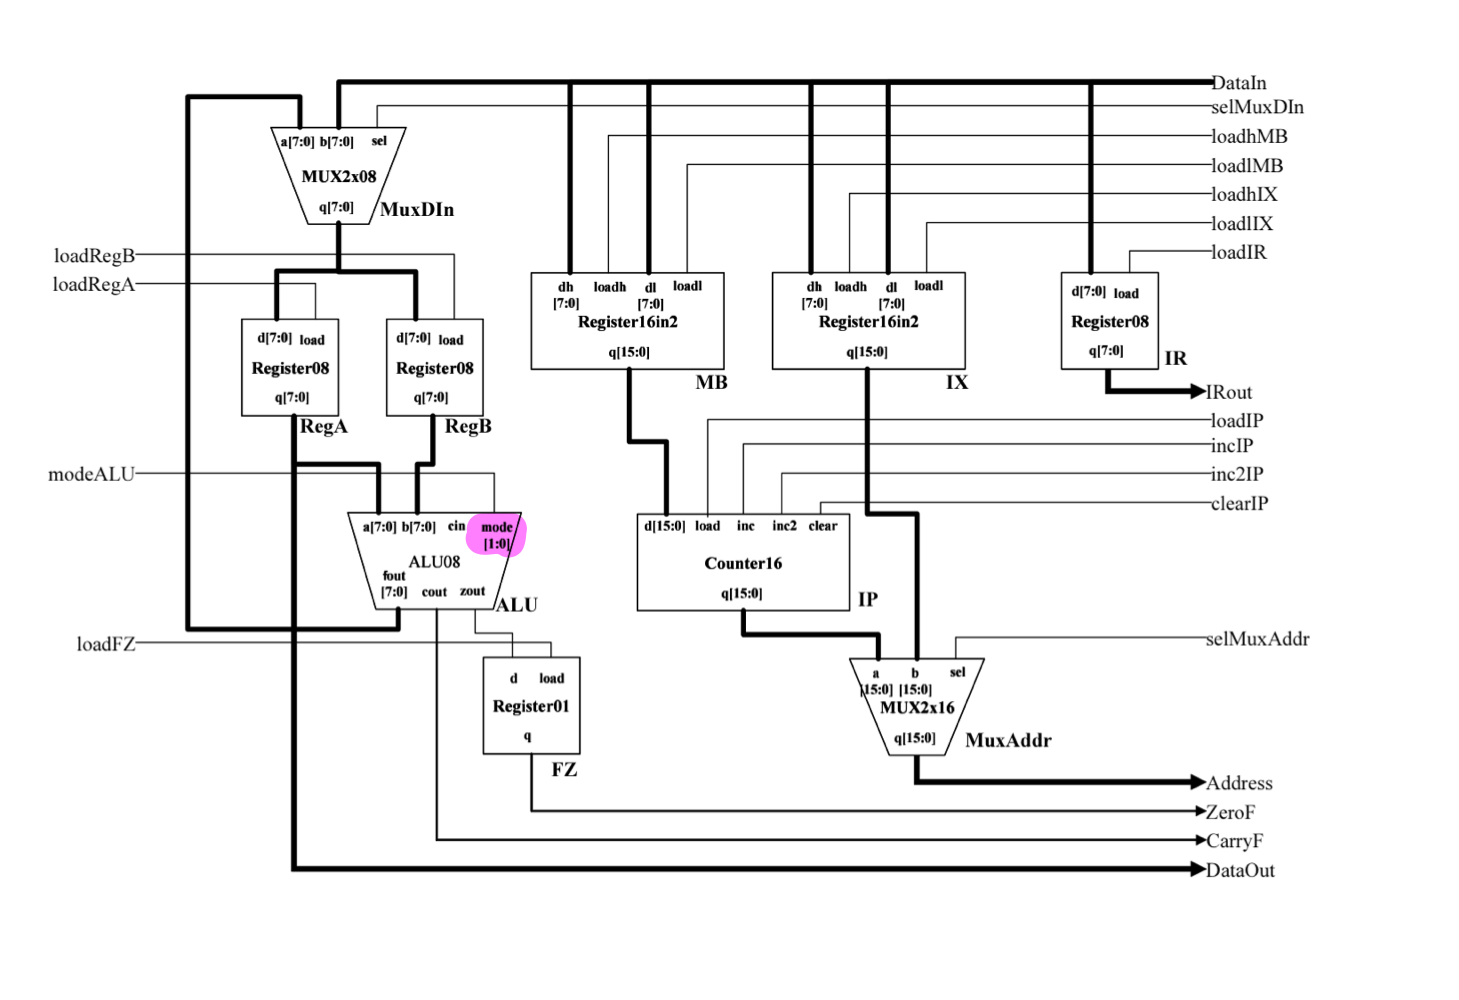
\includegraphics[width=1.1\columnwidth]{Tiny_datapath.png}
      \caption{Tiny-Processorのデータパス}
      \label{fig:a}
  \end{minipage}
  \begin{minipage}[b]{0.49\columnwidth}
      \centering
      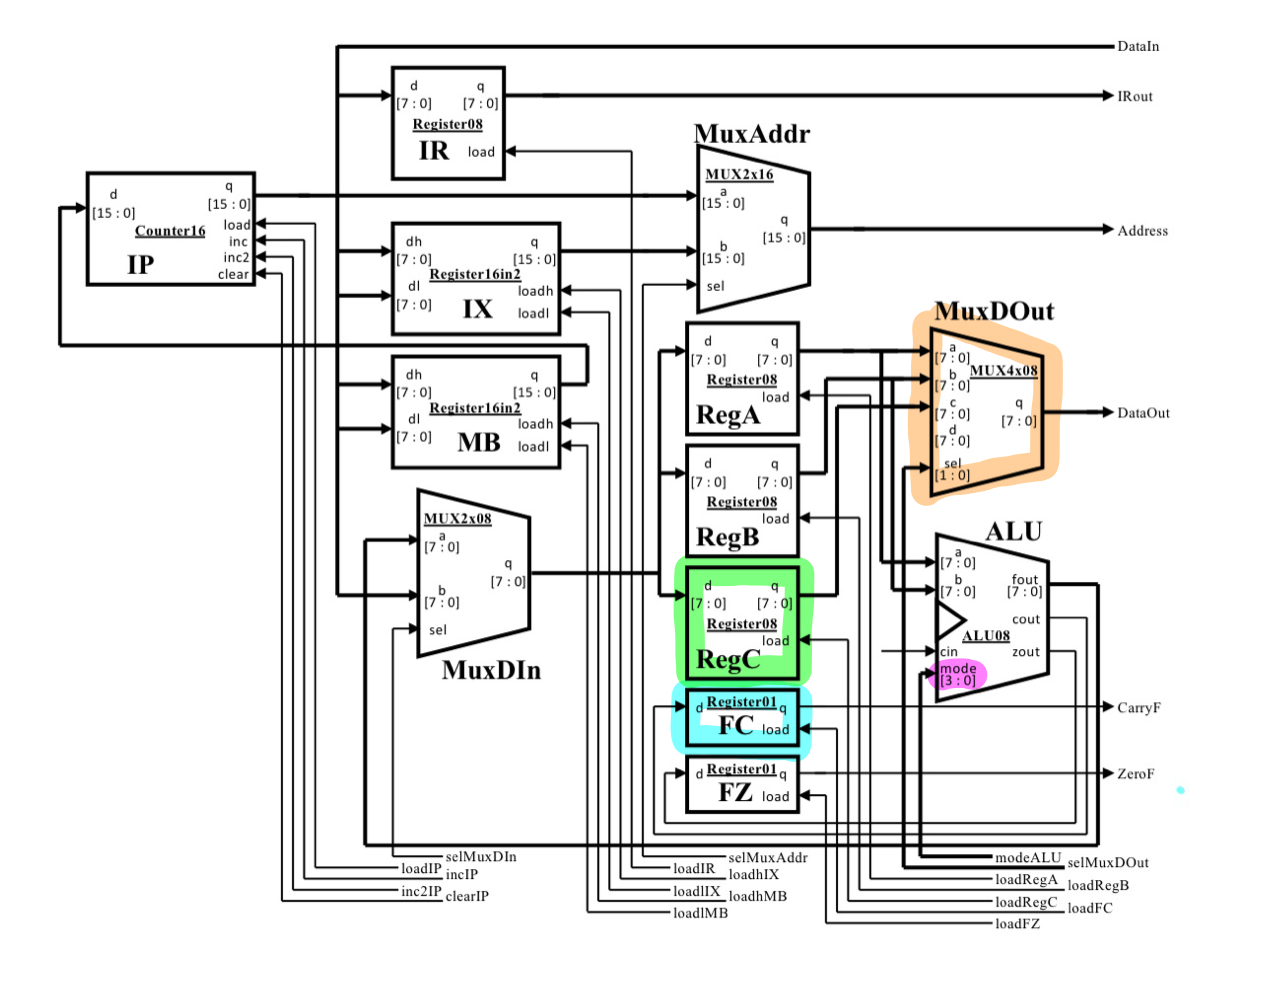
\includegraphics[width=1.1\columnwidth]{C_datapath.png}
      \caption{C-Processorのデータパス}
      \label{fig:b}
  \end{minipage}
  \end{figure}
\\この二つのデータパスの違いを明確にするために色付けをした.以下でそれぞれの違いについて述べる.
\begin{itemize}
  \item 図1のピンクに塗った部分はALUの入力modeを表す.Tiny-Processorではmodeは2ビットの入力として設計されている.図2のピンクで塗った部分は
  C-Processorの同じくALUの入力modeである.C-ProcessorではTiny-Processorよりも機能が増えており,modeの入力が4ビットに増加している.
  \item 図2の緑で塗った部分はRegCであり,C-Processorで追加されている.入力は新たに追加されたloadRegC以外はRegA,RegBと同じである.このレジスタCはSTDI命令の際に使用される.詳細な説明は2で記述する.
  \item 図2の青色で塗った部分はFCであり,C-Processorで追加されている.入力は新たに追加されたloadFCとALUの出力であるcoutで,出力はq即ちCarryFである.これはALUの演算の結果,桁上りが発生したかを判定する.これからCarryFという信号が得られ,JPC命令に利用される.
  \item 図2のオレンジで塗った部分はMuxDOutであり,4入力のマルチプレクサである.ただし,4入力の内3つしか使っておらずその3つの入力はRegA,RegB,RegCの出力である.また,4つの入力の内どの値を出力するかを決定する2ビットのselMuxDOutを追加した.
  そして出力がDataOutとなる.Tiny-ProcessorではRegAの出力がDataOutとなっていたが,C-Processorでは三つのレジスタからマルチプレクサで選択してDataOutを決定している.
\end{itemize}
\clearpage
\section{STDI命令のデータの流れ}
以下の図3は1の図2で示したC-Processorのデータパスに,STDI命令を実行する際のデータの流れを追加したものである.
\begin{figure}[h]
  \centering
  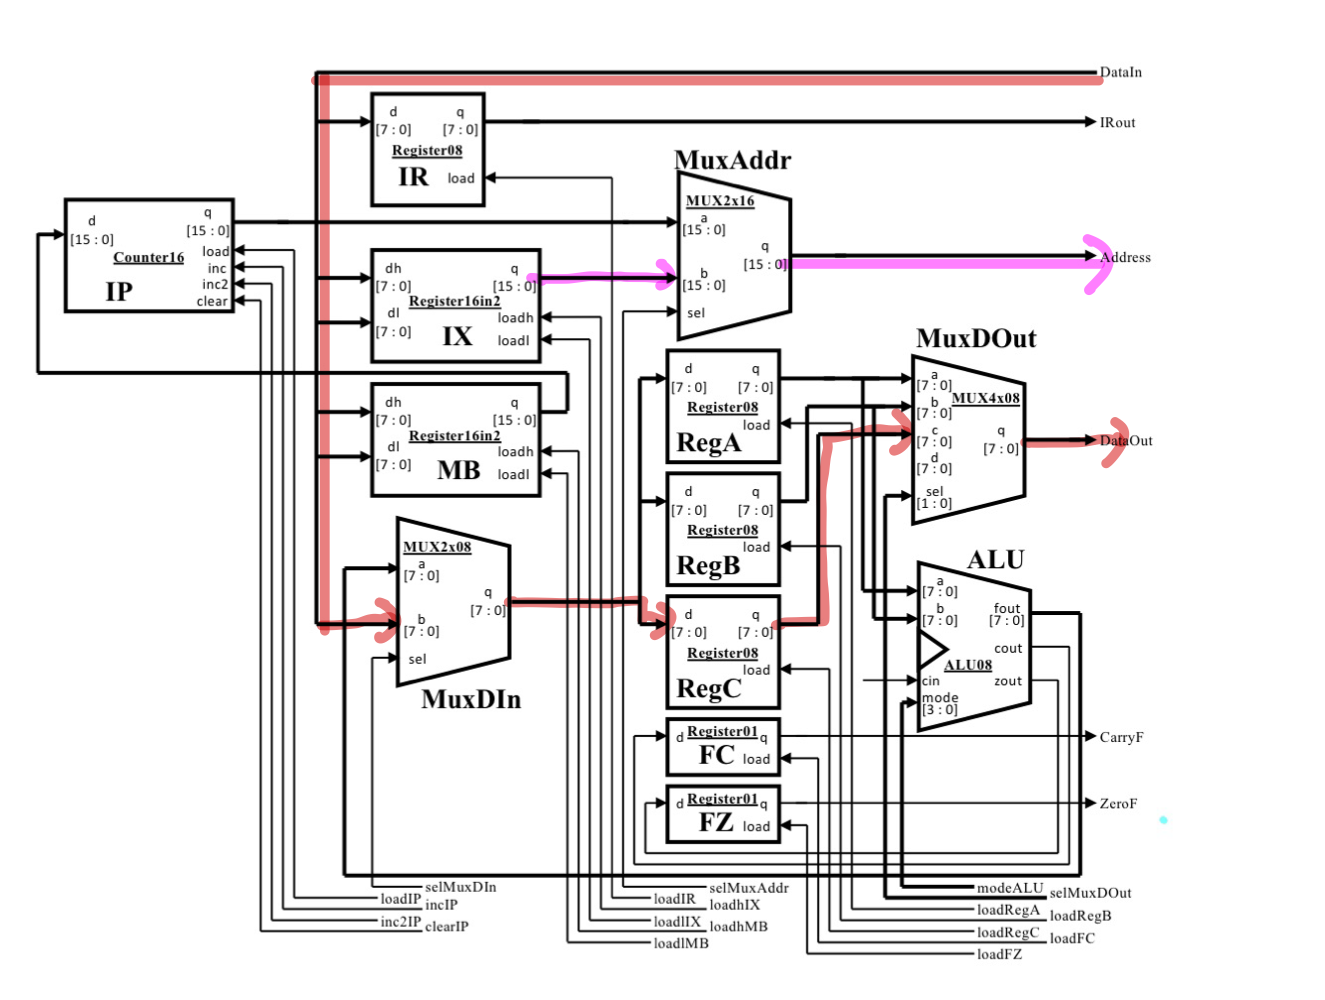
\includegraphics[width = 12cm]{STDI.png}
  \caption{C-ProcessorにおけるSTDI命令のデータの流れ}  
\end{figure}
\\ピンクの矢印はアドレス,赤の矢印はデータの流れを表している.STDI命令は以下の流れで実行される.
\begin{enumerate}
  \item STDI命令が実行される前にIXにアドレスが格納される.
  \item DataInからデータが読み込まれ,レジスタCにその値が格納される.
  \item MuxDOutによってcが選択され,またMuxAddrによってbが選択されることによってIXに入っていたアドレスにDataInの値が即値で格納される.
\end{enumerate}
\clearpage
\section{外部出力信号用ジョンソンカウンタと内部制御信号用ジョンソンカウンタ}
\subsection{外部出力用ジョンソンカウンタ}
C-Processorの外部出力用ジョンソンカウンタは以下のようになる.
\begin{figure}[h]
  \centering
  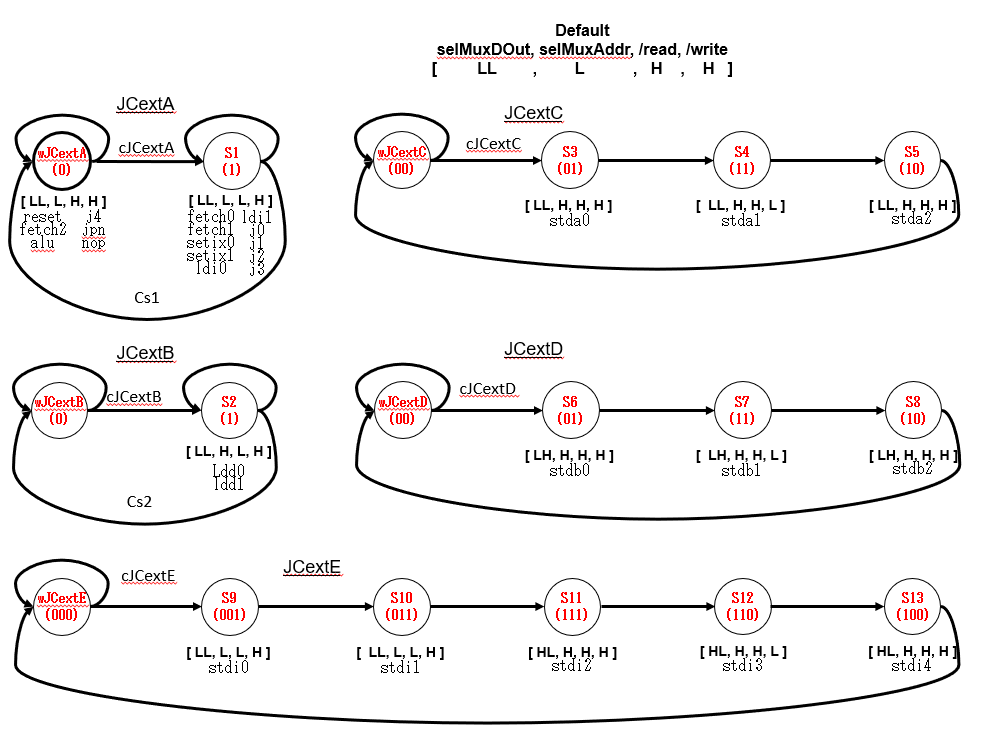
\includegraphics[width = 8cm]{ext.png}
  \caption{外部出力用ジョンソンカウンタ}
\end{figure}
\\外部出力用ジョンソンカウンタはメモリのアクセスに関係する信号を制御する.Tiny-Processorから,STDB命令とSTDI命令を制御するためのジョンソンカウンタを追加した.
そしてselMuxDOut,selMuxAddr,/read,/writeの4つの信号の値をそれぞれの状態に合わせて変動した.
\subsection{内部出力用ジョンソンカウンタ}
C-Processorの内部出力用ジョンソンカウンタは以下のようになる.
\begin{figure}[h]
  \centering
  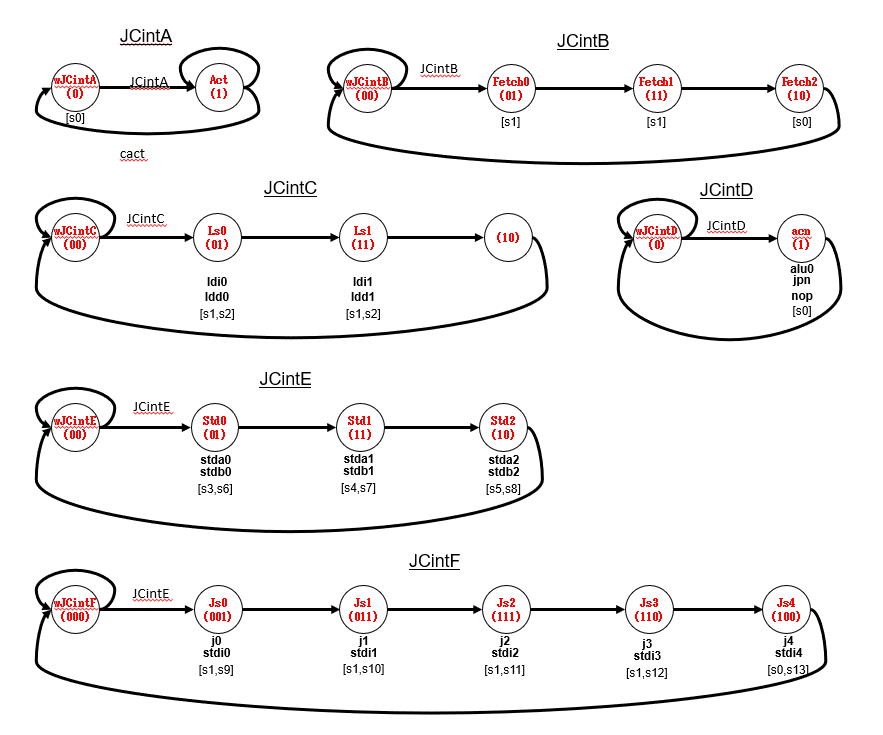
\includegraphics[width = 8cm]{int.png}
  \caption{内部出力用ジョンソンカウンタ}
\end{figure}
\\内部出力用ジョンソンカウンタはレジスタのロード信号やマルチプレクサの選択信号を制御する.
命令の種類即ちIRの値と内部出力用ジョンソンカウンタの値を用いて,外部出力脱出用信号,内部出力脱出用信号,脱出信号以外の条件を作成した.
以下はその条件を表す.
\begin{figure}[h]
  \centering
  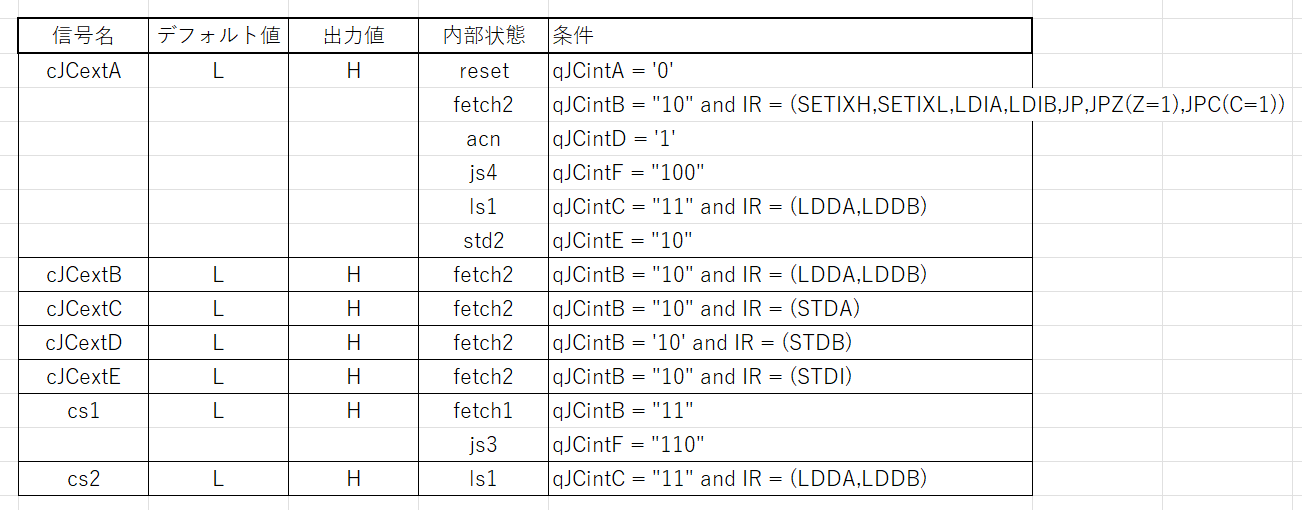
\includegraphics[width = 12cm]{cJCext.png}
  \caption{外部出力脱出信号の条件}
\end{figure}
\begin{figure}[h]
  \centering
  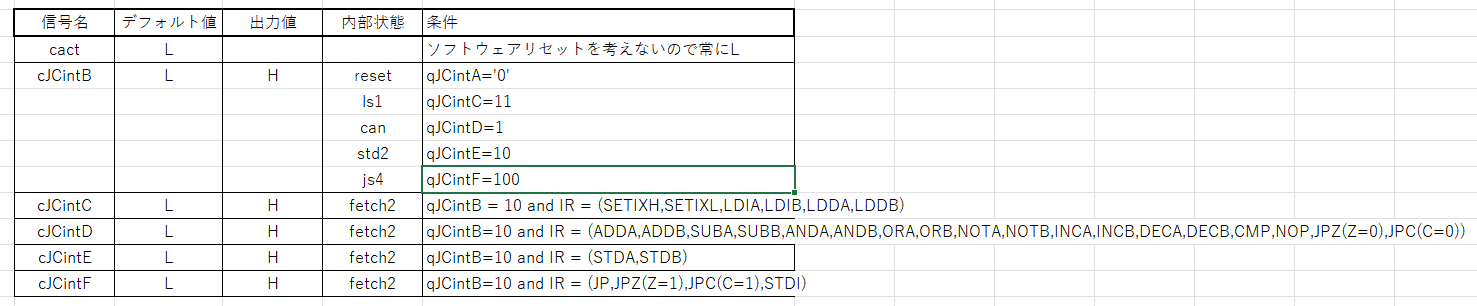
\includegraphics[width = 12cm]{cJCint.png}
  \caption{内部出力脱出信号の条件}
\end{figure}
\begin{figure}[h]
  \centering
  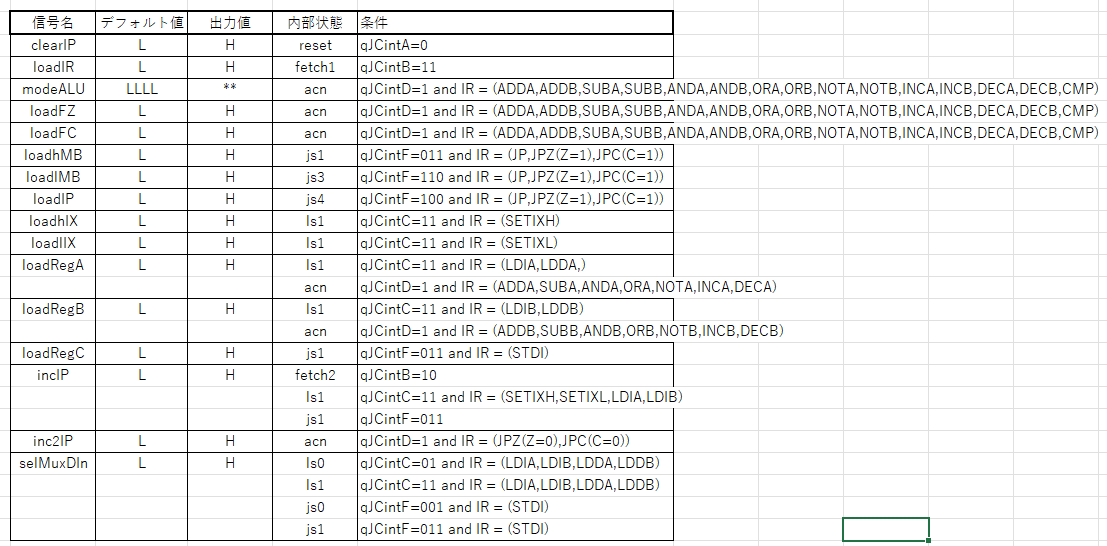
\includegraphics[width = 12cm]{others.png}
  \caption{脱出信号以外の条件}
\end{figure}
\clearpage
\section{拡張課題}
\subsection{拡張課題a:プロセッサ命令セットの拡張}
今回私が追加した命令セットは論理シフトである.いかにその仕様を示す.
\begin{table}[h]
  \centering
  \begin{tabular}{|c||c|c|c|c|}
    \hline
    命令 & オペランド & サイズ & コード\\\hline
    SLLA & id & 1 word & 11000000\\\hline
    SRLA & id & 1 word & 11000001 \\\hline
    SLLB & id & 1 word & 11001000 \\\hline
    SRLB & id & 1 word & 11001001 \\\hline
  \end{tabular}
  \caption{追加した命令}
\end{table}
この4命令は,第一オペランドで即値により指定した数値分レジスタAまたはレジスタBを論理シフトするものである.
これはALUの演算の処理を切り替える4ビットのベクトルmodeALUで未使用の部分を使用して実装した.
したがって,このシフト命令を追加した後のmodeALUの処理は以下のようになる.
\begin{table}[h]
  \centering
  \begin{tabular}{|c|c||c|c||c|c||c|c|}
    \hline
    LLLL & A + B & LHLL & not A & HLLL & not B & HHLL & sllb\\\hline
    LLLH & A - B & LHLH & A + 1 & HLLH  & B + 1 & HHLH & srlb\\\hline
    LLHL & A and B & LHHL & A - 1 & HLHL  & B - 1 & HHHL & 未使用\\\hline
    LLHH & A or B & LHHH & slla & HLHH & srla & HHHH & 未使用\\\hline
  \end{tabular}
  \caption{シフト命令を追加した後のmodeALUの処理}
\end{table}
\\また,ALUが即値を扱えるようにするために入力としてレジスタCを追加した.追加後のデータパスアーキテクチャ図は以下のようになる.
\begin{figure}[h]
  \centering
  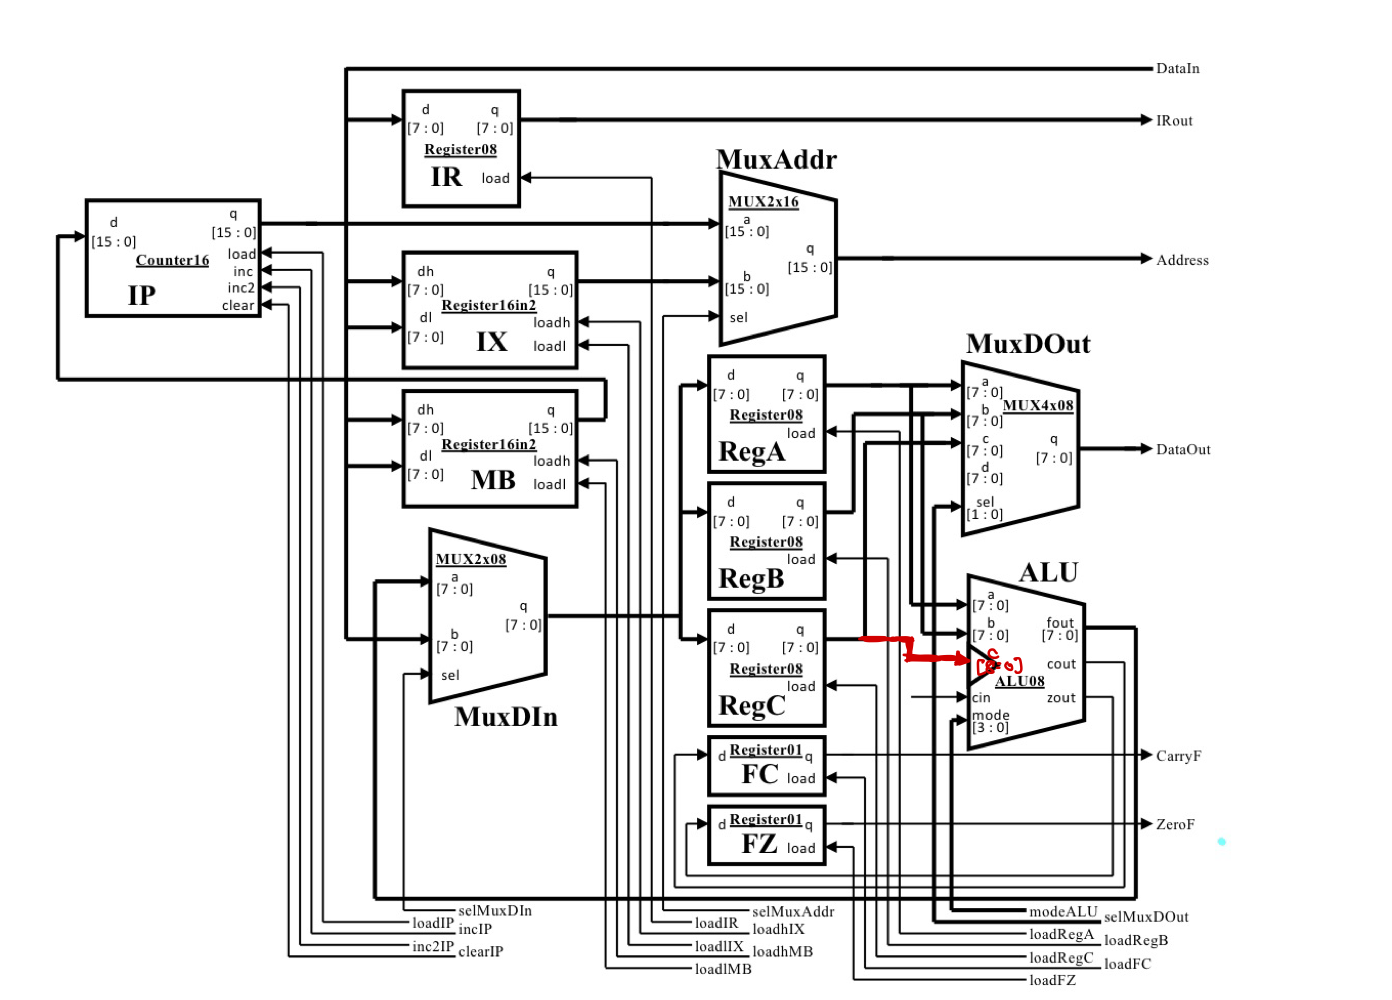
\includegraphics[width = 8cm]{improvedatapath.png}
  \caption{追加後のデータパスアーキテクチャ図}
\end{figure}
赤色の矢印が新たに追加したレジスタCからALUへの入力である.\\
また,SLLA,SRLAの外部出力用ジョンソンカウンタとしてwJextFを,SLLB,SRLB用の外部出力用ジョンソンカウンタとしてwJextGを追加した.
これらはどちらも2ビットのジョンソンカウンタで実装した.したがって,追加後の外部出力用のジョンソンカウンタは以下のようになる.
\clearpage
\begin{figure}[h]
  \centering
  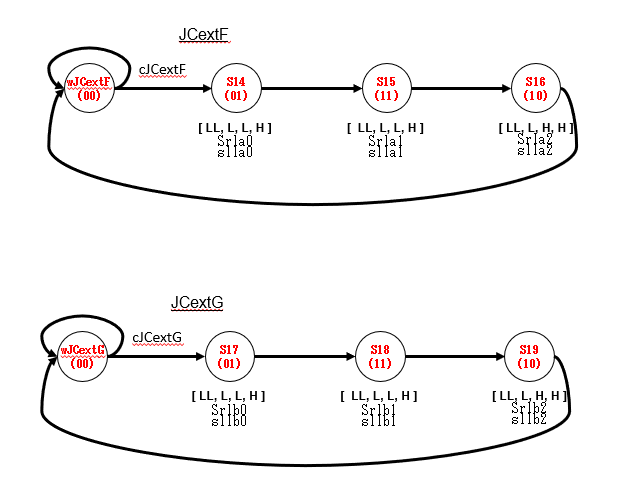
\includegraphics[width = 8cm]{improveext.png}
  \caption{追加後の内部出力用ジョンソンカウンタ}
\end{figure}
そしてメモリアクセス用の信号の条件に上記の内容を追加した.
また,内部出力用のジョンソンカウンタは新たに追加せずJCintCを利用して実装した.即ち,追加したシフト命令はcJCintCはLDIA,LDIBと同じ内部出力用ジョンソンカウンタを使用して
脱出信号等を制御した.したがって,図6から図8の条件にさらにシフト命令用の条件を追加した.\\
具体的なシフトの処理は,NUMETRIC\_STDライブラリを使用し,8ビットのベクトルであるcを整数に変換し,それを使用してaまたはbを論理シフトするという方法で実装した.
以下では実行結果を示す.
\begin{figure}[h]
  \centering
  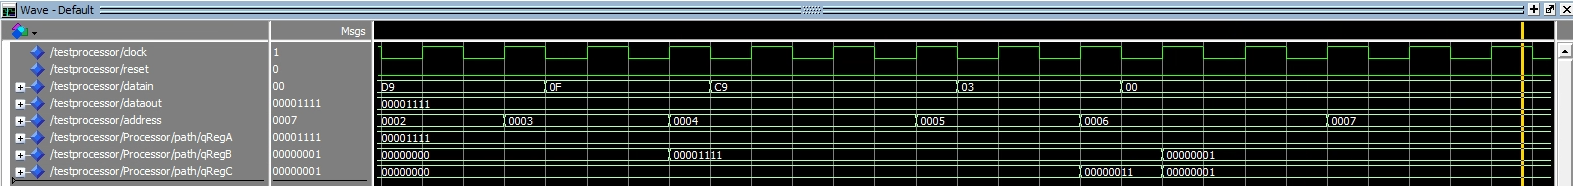
\includegraphics[width = 16cm]{result.png}
  \caption{シフト命令の実行結果}
\end{figure}
\\これは,レジスタA,Bのどちらにも00001111が格納されている際に"SRLB 03"を実行した際の波形である.addressが0006の際にレジスタCに3を表す
00000011が入り,その後Bが右に3ビットシフトされてレジスタBに00000001が格納されている.
\subsection{拡張課題b:演算機の改善}
\begin{enumerate}
  \item まず,桁上げ先見加算器について説明する.桁上げ先見加算器は最大の遅延がO(logn)の加算器であり,演算対象の桁数が多い場合に効率よく計算が実行できる.
  今回はまず4ビットの桁上げ先見加算器について記述し,それを組み合わせて8ビット,16ビットの加算器を作成する.
  \\桁上げ先見加算器はまず入力xとyに対して桁上げ生成関数Gと桁上げ伝播関数Pを計算する.計算式は以下のようになる.
  \[
    g_i = x_i \land y_i
  \]
  \[p_i = x_i \oplus y_i\]
  iは4ビットの内の何桁目かを表しており,例えば$g_2$は下から三桁目を表している.そして,これらの値を用いて以下のように出力sと桁上げ出力cを計算する.
  \[
    s_i = p_i \oplus c_{i-1}
  \]
  \[c_i = g_i \lor (p_i \land c_{i-1}) \]
  この漸化式に代入を繰り返していくと,最終的に$x_i$と$y_i$と$c_{-1}$のみで表すことができるようになる.したがって,RCAとは違い,下位ビットの桁上りを待つ必要がなくなる.
  \item 今回は上記の方法でまず4ビットのLCAを設計した.そして,それを二つ利用して8ビットのLCAを実現した.
  具体的には,一つのLCAには入力の下位4ビット,$c_{-1}$を入力とし,もう一つのLCAには入力の上位4ビット,下位ビット用のLCAが出力したキャリーを入力とした.
  そして最後に結果を結合することにより計算を実現した.
  16bit桁上げ先見加算器も8ビットLCAに対して同様にすることで実装した.
  \item 
\end{enumerate}
\section{感想}
今回の課題を通してCPUがどのように設計されているのかについて学ぶことができて非常に興味深かった.特に,内部出力用ジョンソンカウンタと外部出力用ジョンソンカウンタを分けて
信号を制御している部分がとても驚いた.これまでの実験を通して問題を分割することの重要性を再三認識してきたが,また改めてその重要性を感じることができた.
\end{document}